\documentclass[11pt,a4paper]{article}

% ============================================================
% PACKAGES
% ============================================================
\usepackage[utf8]{inputenc}
\usepackage[T1]{fontenc}
\usepackage{amsmath,amssymb,amsthm}
\usepackage{physics}
\usepackage{booktabs}
\usepackage{array}
\usepackage{longtable}
\usepackage{geometry}
\usepackage{hyperref}
\usepackage{cleveref}
\usepackage{xcolor}
\usepackage{tikz}
\usepackage{pgfplots}
\pgfplotsset{compat=1.18}
\usetikzlibrary{patterns,arrows.meta,positioning,decorations.pathmorphing,shapes.geometric}

\geometry{margin=1in}

% ============================================================
% CUSTOM COMMANDS
% ============================================================
\newcommand{\Mpl}{\bar{M}_{\mathrm{Pl}}}
\newcommand{\MplOrig}{M_{\mathrm{Pl}}}
\newcommand{\Mfive}{M_5}
\newcommand{\Rxi}{R_\xi}
\newcommand{\mgap}{m_{\mathrm{gap}}}
\newcommand{\mb}{m_b}
\newcommand{\MZ}{M_Z}
\newcommand{\GeV}{\,\mathrm{GeV}}
\newcommand{\TeV}{\,\mathrm{TeV}}
\newcommand{\tagD}{\textbf{[D]}}
\newcommand{\tagDc}{\textbf{[Dc]}}
\newcommand{\tagI}{\textbf{[I]}}
\newcommand{\tagBL}{\textbf{[BL]}}
\newcommand{\tagP}{\textbf{[P]}}
\newcommand{\tagOPEN}{\textbf{[OPEN]}}
\newcommand{\emark}{\textcolor{green!70!black}{\checkmark}}

% ============================================================
% THEOREM ENVIRONMENTS
% ============================================================
\theoremstyle{definition}
\newtheorem{definition}{Definition}[section]
\newtheorem{hypothesis}{Hypothesis}[section]
\newtheorem{candidate}{Candidate}[section]

\theoremstyle{plain}
\newtheorem{proposition}{Proposition}[section]
\newtheorem{theorem}{Theorem}[section]
\newtheorem{lemma}{Lemma}[section]

\theoremstyle{remark}
\newtheorem{remark}{Remark}[section]

% ============================================================
% DOCUMENT
% ============================================================
\begin{document}

\title{\textbf{Derivation v27: Brane Mass from Brane Tension}\\[0.5em]
\large BLOCK-003 Gravity Program --- $\mb$ from $\sigma$ + Topological Pinning Candidate}
\author{EDC Collaboration}
\date{February 2026}
\maketitle

\begin{abstract}
We construct a minimal-dimensional and action-level connection between the brane-localized
mass parameter $\mb$ (introduced in v26) and the brane tension $\sigma$. Starting from
the dimensional ansatz $\mb = \lambda\,\sigma/\Mfive^3$, we express the dimensionless
control parameter $b \equiv \mb L$ in terms of $\sigma$, $\Mfive$, $L$, and $\Mpl$.
We explore a \emph{topological pinning candidate} where $\lambda$ is discretized
($\lambda = \pi n$ or $2\pi n$) due to orbifold/holonomy constraints. The spectral
equation from v26 is re-expressed in terms of these parameters, mapping precisely
where the gap becomes fixed. All quantities are rigorously tagged: the relation
$\mb = \lambda\sigma/\Mfive^3$ achieves \tagDc{} status (one free parameter $\lambda$),
while the gap prediction remains \tagI{}+\tagBL{} until $L$ or $\lambda$ is independently
determined. Numerical verification confirms the limiting behaviors and explores
the discrete spectrum for quantized $\lambda$.
\end{abstract}

\tableofcontents
\newpage

% ============================================================
% SECTION 1: INTRODUCTION AND EPISTEMIC FRAMEWORK
% ============================================================
\section{Introduction and Epistemic Framework}
\label{sec:intro}

\subsection{Context from v26}

In derivation v26, we established the \emph{Gap Derivability Program}:
\begin{itemize}
\item A brane-localized mass term generates Robin boundary conditions
\item The transcendental spectrum $\tan(m_n L) = -\mb/m_n$ was derived \tagD{}
\item The gap bounds $\pi/2L < \mgap < \pi/L$ were established \tagD{}
\item The gap status remained \tagI{}+\tagBL{} because $L$ and $\mb$ were not derived
\end{itemize}

\subsection{Goal of This Note}

This derivation addresses the question:
\begin{quote}
\textbf{Can $\mb$ be derived from EDC-internal parameters, specifically the brane tension $\sigma$?}
\end{quote}

We construct:
\begin{enumerate}
\item A dimensional relation $\mb = \lambda\,\sigma/\Mfive^3$
\item An action-level justification for this relation
\item The dimensionless control parameter $b = \mb L$
\item A topological pinning candidate where $\lambda$ is quantized
\end{enumerate}

\subsection{Epistemic Tags}

\begin{table}[htbp]
\centering
\caption{Epistemic classification used in this derivation.}
\label{tab:tags}
\begin{tabular}{@{}lll@{}}
\toprule
Tag & Meaning & Status \\
\midrule
\tagD{} & Fully derived (no free parameters) & Best \\
\tagDc{} & Derived with one calibration/parameter & Good \\
\tagP{} & Postulated (hypothesis/candidate) & Uncertain \\
\tagI{} & Identified with observable & External \\
\tagBL{} & Baseline (measured input) & External \\
\tagOPEN{} & Unresolved & Gap \\
\bottomrule
\end{tabular}
\end{table}

% ============================================================
% SECTION 2: DIMENSIONAL ANALYSIS
% ============================================================
\section{Dimensional Analysis: $\mb$ from $\sigma$}
\label{sec:dimensional}

\subsection{Available Scales}

The EDC brane setup provides the following mass scales:
\begin{align}
[\sigma] &= M^4 \quad \text{(brane tension)} \label{eq:dim-sigma} \\
[\Mfive] &= M \quad \text{(5D Planck mass)} \label{eq:dim-M5} \\
[L] &= M^{-1} \quad \text{(compactification length)} \label{eq:dim-L} \\
[\Mpl] &= M \quad \text{(4D reduced Planck mass)} \label{eq:dim-Mpl}
\end{align}

\subsection{Target Dimension}

The brane mass parameter has dimension:
\begin{equation}
[\mb] = M
\label{eq:dim-mb}
\end{equation}

\subsection{Dimensional Candidates}

We seek combinations of $\sigma$, $\Mfive$, and $L$ that yield dimension $M$:
\begin{align}
\frac{\sigma}{\Mfive^3} &: \quad \frac{M^4}{M^3} = M \quad \emark \label{eq:cand-1} \\
\sigma L^3 &: \quad M^4 \cdot M^{-3} = M \quad \emark \label{eq:cand-2} \\
\frac{\sigma L}{\Mfive^2} &: \quad \frac{M^4 \cdot M^{-1}}{M^2} = M \quad \emark \label{eq:cand-3}
\end{align}

\subsection{Primary Candidate}

The most natural choice (involving only $\sigma$ and $\Mfive$, without $L$) is:
\begin{equation}
\boxed{\mb = \lambda \, \frac{\sigma}{\Mfive^3}}
\label{eq:mb-primary}
\end{equation}
where $\lambda$ is a dimensionless coefficient.

\begin{proposition}[Dimensional Consistency]
\label{prop:dim-consistency}
The relation \cref{eq:mb-primary} is dimensionally consistent:
\begin{equation}
[\mb] = \frac{[\sigma]}{[\Mfive^3]} = \frac{M^4}{M^3} = M \quad \emark
\label{eq:dim-check}
\end{equation}
\end{proposition}

\subsection{Physical Interpretation}

The ratio $\sigma/\Mfive^3$ has a natural interpretation:
\begin{itemize}
\item $\sigma$ is the energy density localized on the brane
\item $\Mfive^3$ sets the 5D gravitational coupling scale
\item $\sigma/\Mfive^3$ measures the ``strength'' of brane effects relative to bulk gravity
\end{itemize}

\subsection{Status of the Dimensional Relation}

\begin{equation}
\mb = \lambda \, \frac{\sigma}{\Mfive^3} \quad \tagDc{}
\label{eq:mb-status}
\end{equation}

The relation is \tagDc{} because:
\begin{itemize}
\item The dimensional structure is derived \tagD{}
\item The coefficient $\lambda$ remains undetermined \tagOPEN{}
\end{itemize}

% ============================================================
% SECTION 3: ACTION-LEVEL DERIVATION
% ============================================================
\section{Action-Level Derivation}
\label{sec:action}

\subsection{5D Action with Brane}

The total action consists of bulk and brane contributions:
\begin{equation}
S = S_{\mathrm{bulk}} + S_{\mathrm{brane}}
\label{eq:total-action}
\end{equation}

\subsubsection{Bulk Action}

The 5D bulk action for a scalar field $\Phi$:
\begin{equation}
S_{\mathrm{bulk}} = -\frac{1}{2}\int d^5x \sqrt{-g^{(5)}} \, g^{MN}\partial_M\Phi\partial_N\Phi
\label{eq:bulk-action}
\end{equation}

\subsubsection{Brane Action}

The brane at $\xi = L$ carries tension $\sigma$ and couples to bulk fields:
\begin{equation}
S_{\mathrm{brane}} = -\int d^4x \sqrt{-\gamma} \left[ \sigma + \frac{1}{2}\mu\,\Phi^2 \right]_{\xi=L}
\label{eq:brane-action}
\end{equation}
where $\gamma_{\mu\nu}$ is the induced metric and $\mu$ is a brane-localized mass-squared parameter.

\subsection{Brane-Induced Boundary Operator}

The key question is: how does $\sigma$ generate the brane mass $\mb$?

\subsubsection{Mechanism: Tension-Field Coupling}

Consider the gravitational backreaction of the brane tension. The Israel junction
condition gives:
\begin{equation}
[K_{\mu\nu}] - \gamma_{\mu\nu}[K] = -\kappa_5^2 \, \sigma \, \gamma_{\mu\nu}
\label{eq:junction}
\end{equation}
where $K_{\mu\nu}$ is the extrinsic curvature and $\kappa_5^2 = 1/\Mfive^3$.

\subsubsection{Field-Dependent Correction}

When a bulk scalar $\Phi$ is present, the effective tension becomes field-dependent:
\begin{equation}
\sigma_{\mathrm{eff}} = \sigma + \Delta\sigma(\Phi)
\label{eq:effective-tension}
\end{equation}

Expanding to quadratic order in $\Phi$:
\begin{equation}
\Delta\sigma(\Phi) = \frac{1}{2}\alpha_\sigma \, \Phi^2 + O(\Phi^4)
\label{eq:delta-sigma}
\end{equation}
where $\alpha_\sigma$ is a coupling coefficient with dimension $[M^2]$.

\subsubsection{Natural Scale for $\alpha_\sigma$}

The only available scales are $\sigma$ and $\Mfive$. Dimensional analysis gives:
\begin{equation}
\alpha_\sigma = c \, \frac{\sigma}{\Mfive^2}
\label{eq:alpha-sigma}
\end{equation}
where $c$ is a dimensionless $O(1)$ coefficient.

\subsubsection{Effective Brane Mass Term}

Substituting into \cref{eq:brane-action}:
\begin{equation}
S_{\mathrm{brane}} \supset -\frac{1}{2}\int d^4x \sqrt{-\gamma} \, \alpha_\sigma \, \Phi^2\big|_{\xi=L}
\label{eq:effective-mass-term}
\end{equation}

Comparing with the standard form $S_{\mathrm{brane}} \supset -\frac{1}{2}\int d^4x \sqrt{-\gamma} \, \mb \, \Phi^2$:
\begin{equation}
\mb = \alpha_\sigma = c \, \frac{\sigma}{\Mfive^2}
\label{eq:mb-from-alpha}
\end{equation}

\subsection{Reconciling Dimensions}

Wait---\cref{eq:mb-from-alpha} gives $[\mb] = M^4/M^2 = M^2$, but we need $[\mb] = M$.

This indicates that the simple $\Phi^2$ term in the action must be reinterpreted.

\subsubsection{Correct Action Structure}

The brane-localized mass term should be:
\begin{equation}
S_{\mathrm{brane}} \supset -\frac{1}{2}\int d^4x \sqrt{-\gamma} \, \mb \, \Phi^2
\label{eq:correct-mass-term}
\end{equation}
where $[\mb] = M^1$ (mass dimension 1), and $[\Phi] = M^{3/2}$ in 5D.

Actually, for a canonically normalized 5D scalar, $[\Phi] = M^{3/2}$, so:
\begin{equation}
[\mb\,\Phi^2] = M \cdot M^3 = M^4
\label{eq:dim-check-2}
\end{equation}
which integrates to give dimension $[M^4 \cdot L^{-4}] = M^0$ in 4D. This is consistent.

\subsubsection{Proper Derivation}

The brane coupling to $\Phi$ arises from the tension's dependence on bulk fields.
Using the relation:
\begin{equation}
\kappa_5^2 = \frac{1}{\Mfive^3}
\label{eq:kappa5}
\end{equation}

The natural scale for brane-induced mass is:
\begin{equation}
\mb \sim \kappa_5^2 \cdot \sigma = \frac{\sigma}{\Mfive^3}
\label{eq:mb-natural}
\end{equation}

Therefore:
\begin{equation}
\boxed{\mb = \lambda \, \frac{\sigma}{\Mfive^3} \quad \text{where } \lambda \sim O(1)}
\label{eq:mb-final}
\end{equation}

\subsection{Action-Level Status}

\begin{table}[htbp]
\centering
\caption{Derivation status of $\mb = \lambda\sigma/\Mfive^3$.}
\label{tab:mb-status}
\begin{tabular}{@{}lll@{}}
\toprule
Component & Status & Tag \\
\midrule
Dimensional structure & Derived & \tagD{} \\
Scaling with $\sigma$ & Derived from coupling & \tagD{} \\
Scaling with $\Mfive^{-3}$ & From $\kappa_5^2$ & \tagD{} \\
Coefficient $\lambda$ & Undetermined & \tagOPEN{} \\
\midrule
Overall relation & Derived with 1 parameter & \tagDc{} \\
\bottomrule
\end{tabular}
\end{table}

% ============================================================
% SECTION 4: DIMENSIONLESS CONTROL PARAMETER
% ============================================================
\section{Dimensionless Control Parameter $b = \mb L$}
\label{sec:dimensionless}

\subsection{Definition}

From v26, the gap is controlled by the dimensionless parameter:
\begin{equation}
b \equiv \mb \cdot L
\label{eq:b-def}
\end{equation}

The transcendental spectral equation is:
\begin{equation}
\tan(x_n) = -\frac{b}{x_n}, \qquad x_n = m_n L
\label{eq:spectral}
\end{equation}

\subsection{Expression in Terms of $\sigma$, $\Mfive$, $L$}

Substituting $\mb = \lambda\sigma/\Mfive^3$:
\begin{equation}
b = \mb L = \lambda \, \frac{\sigma L}{\Mfive^3}
\label{eq:b-sigma}
\end{equation}

\subsection{Using the Bridge Relation}

From v23/v15, the bridge relation is:
\begin{equation}
\Mpl^2 = \Mfive^3 \cdot L \quad \tagD{}
\label{eq:bridge}
\end{equation}

Solving for $\Mfive^3$:
\begin{equation}
\Mfive^3 = \frac{\Mpl^2}{L}
\label{eq:M5-from-bridge}
\end{equation}

Substituting into \cref{eq:b-sigma}:
\begin{equation}
b = \lambda \, \frac{\sigma L}{\Mpl^2/L} = \lambda \, \frac{\sigma L^2}{\Mpl^2}
\label{eq:b-Mpl}
\end{equation}

\begin{equation}
\boxed{b = \mb L = \lambda \, \frac{\sigma L^2}{\Mpl^2} \quad \tagDc{}}
\label{eq:b-final}
\end{equation}

\subsection{Alternative Forms}

\subsubsection{In Terms of $\Mfive$ and $L$}

Using $\Mpl^2 = \Mfive^3 L$:
\begin{equation}
b = \lambda \, \frac{\sigma L^2}{\Mfive^3 L} = \lambda \, \frac{\sigma L}{\Mfive^3}
\label{eq:b-M5}
\end{equation}

\subsubsection{In Terms of $\sigma$ and $\Mpl$ Only}

If we use $L = \Mpl^2/\Mfive^3$:
\begin{equation}
b = \lambda \, \frac{\sigma}{\Mfive^3} \cdot \frac{\Mpl^2}{\Mfive^3} = \lambda \, \frac{\sigma \Mpl^2}{\Mfive^6}
\label{eq:b-M5-6}
\end{equation}

\subsection{Scaling Relations}

From \cref{eq:b-final}:
\begin{align}
b &\propto \sigma \label{eq:b-scale-sigma} \\
b &\propto L^2 \label{eq:b-scale-L} \\
b &\propto \Mpl^{-2} \label{eq:b-scale-Mpl}
\end{align}

\subsection{Derivative Relations}

The sensitivity of $b$ to parameter changes:
\begin{equation}
\frac{\partial b}{\partial \sigma} = \lambda \, \frac{L^2}{\Mpl^2}
\label{eq:db-dsigma}
\end{equation}

\begin{equation}
\frac{\partial b}{\partial L} = 2\lambda \, \frac{\sigma L}{\Mpl^2}
\label{eq:db-dL}
\end{equation}

\begin{equation}
\frac{\partial b}{\partial \Mpl} = -2\lambda \, \frac{\sigma L^2}{\Mpl^3}
\label{eq:db-dMpl}
\end{equation}

In logarithmic form:
\begin{equation}
\frac{d\ln b}{d\ln \sigma} = 1, \qquad \frac{d\ln b}{d\ln L} = 2, \qquad \frac{d\ln b}{d\ln \Mpl} = -2
\label{eq:log-derivatives}
\end{equation}

\subsection{Gap Dependence}

The first KK mode (gap) satisfies:
\begin{equation}
\tan(x_1) = -\frac{b}{x_1}
\label{eq:gap-eq}
\end{equation}

with:
\begin{equation}
\mgap = \frac{x_1}{L}
\label{eq:gap-from-x1}
\end{equation}

Therefore:
\begin{equation}
\mgap = \frac{x_1(b)}{L} = \frac{x_1(\lambda\sigma L^2/\Mpl^2)}{L}
\label{eq:gap-functional}
\end{equation}

% ============================================================
% SECTION 5: TOPOLOGICAL PINNING CANDIDATE
% ============================================================
\section{Topological Pinning Candidate}
\label{sec:pinning}

\subsection{Motivation}

The coefficient $\lambda$ in $\mb = \lambda\sigma/\Mfive^3$ is currently \tagOPEN{}.
We explore whether $\lambda$ could be \emph{discretized} through topological constraints.

\begin{hypothesis}[Topological Quantization of $\lambda$]
\label{hyp:quantized-lambda}
The coefficient $\lambda$ is not a free continuous parameter but takes discrete values:
\begin{equation}
\lambda = \pi n \quad \text{or} \quad \lambda = 2\pi n, \qquad n \in \mathbb{Z}^+
\label{eq:lambda-quantized}
\end{equation}
due to topological constraints on the brane-bulk coupling.
\end{hypothesis}

\textbf{Status}: \tagP{} (Hypothesis/Candidate)

\subsection{Possible Origins of Quantization}

\subsubsection{Origin 1: Orbifold Parity Projection}

On an $S^1/\mathbb{Z}_2$ orbifold, fields have definite parity under $\xi \to -\xi$.
The boundary operator coupling must respect this symmetry:
\begin{equation}
\int_{\mathrm{brane}} \Phi^2 \quad \text{requires even parity for } \Phi
\label{eq:parity}
\end{equation}

The orbifold projection can introduce factors of $\pi$ in normalization:
\begin{equation}
\frac{1}{2\pi R} \int_{-\pi R}^{\pi R} d\xi \to \frac{1}{\pi R} \int_0^{\pi R} d\xi
\label{eq:orbifold-norm}
\end{equation}

\subsubsection{Origin 2: Holonomy/Winding Number}

If the brane-localized interaction arises from integrating out a bulk field
with non-trivial holonomy around the compact dimension:
\begin{equation}
\oint A_5 \, d\xi = 2\pi n \quad (n \in \mathbb{Z})
\label{eq:holonomy}
\end{equation}

The effective boundary operator inherits quantization:
\begin{equation}
\lambda = \frac{1}{2\pi}\oint A_5 \, d\xi = n
\label{eq:lambda-from-holonomy}
\end{equation}

or with additional factors:
\begin{equation}
\lambda = 2\pi n \quad \text{or} \quad \lambda = \pi n
\label{eq:lambda-variants}
\end{equation}

\subsubsection{Origin 3: Boundary Counterterm from Bulk Integration}

Consider the bulk action integrated up to the brane:
\begin{equation}
S_{\mathrm{eff}} = -\frac{1}{2}\int d^4x \int_0^L d\xi \, (\partial\Phi)^2 + S_{\mathrm{brane}}
\label{eq:bulk-integrated}
\end{equation}

The boundary term from integration by parts:
\begin{equation}
\delta S = -\int d^4x \, \Phi \partial_\xi\Phi \big|_0^L
\label{eq:boundary-term}
\end{equation}

If this is canceled by a brane counterterm proportional to $\sigma$:
\begin{equation}
S_{\mathrm{ct}} = c \, \frac{\sigma}{\Mfive^3} \int d^4x \, \Phi^2\big|_{L}
\label{eq:counterterm}
\end{equation}

The coefficient $c$ could be fixed by requiring cancellation of divergences,
potentially giving a quantized value.

\subsection{Discrete Spectrum for $b$}

If $\lambda = \pi n$:
\begin{equation}
b_n = \pi n \, \frac{\sigma L^2}{\Mpl^2}, \qquad n = 1, 2, 3, \ldots
\label{eq:bn-pi}
\end{equation}

If $\lambda = 2\pi n$:
\begin{equation}
b_n = 2\pi n \, \frac{\sigma L^2}{\Mpl^2}, \qquad n = 1, 2, 3, \ldots
\label{eq:bn-2pi}
\end{equation}

\subsection{Gap Spectrum}

For each discrete $b_n$, the gap is:
\begin{equation}
\mgap^{(n)} = \frac{x_1(b_n)}{L}
\label{eq:gap-n}
\end{equation}

where $x_1(b)$ is the first root of $\tan(x) = -b/x$.

\subsection{Status of Topological Pinning}

\begin{table}[htbp]
\centering
\caption{Status of topological pinning components.}
\label{tab:pinning-status}
\begin{tabular}{@{}lll@{}}
\toprule
Component & Evidence & Tag \\
\midrule
Quantization hypothesis & Plausible & \tagP{} \\
Orbifold origin & Consistent & \tagP{} \\
Holonomy origin & Consistent & \tagP{} \\
Counterterm origin & Speculative & \tagP{} \\
Specific value of $\lambda$ & Not determined & \tagOPEN{} \\
\bottomrule
\end{tabular}
\end{table}

\subsection{What Would Fix the Gap?}

If $\lambda$ is quantized ($\lambda = \pi n$) and $L$ is determined:
\begin{equation}
b = \pi n \, \frac{\sigma L^2}{\Mpl^2} \quad \text{(fixed for given } n, \sigma, L\text{)}
\label{eq:b-fixed}
\end{equation}

The remaining freedom is:
\begin{itemize}
\item Integer $n$ (could be $n = 1$ as minimal choice)
\item Compactification scale $L$ (currently \tagI{}+\tagBL{})
\item Brane tension $\sigma$ (could be EDC-derivable)
\end{itemize}

% ============================================================
% SECTION 6: CONNECTION TO V26 SPECTRAL EQUATION
% ============================================================
\section{Connection to v26 Spectral Equation}
\label{sec:v26-connection}

\subsection{V26 Transcendental Equation}

From derivation v26, with Neumann at $\xi = 0$ and Robin at $\xi = L$:
\begin{equation}
\tan(m_n L) = -\frac{\mb}{m_n} \quad \tagD{}
\label{eq:v26-spectral}
\end{equation}

\subsection{Dimensionless Form}

With $x_n = m_n L$ and $b = \mb L$:
\begin{equation}
\tan(x_n) = -\frac{b}{x_n} \quad \tagD{}
\label{eq:dimensionless-spectral}
\end{equation}

\subsection{$b$ as Function of EDC Parameters}

Substituting $b = \lambda\sigma L^2/\Mpl^2$:
\begin{equation}
\tan(x_n) = -\frac{\lambda\sigma L^2}{\Mpl^2 x_n} \quad \tagDc{}
\label{eq:spectral-sigma}
\end{equation}

\subsection{Gap Formula}

The gap is:
\begin{equation}
\mgap = \frac{x_1(b)}{L} = \frac{x_1(\lambda\sigma L^2/\Mpl^2)}{L}
\label{eq:gap-formula}
\end{equation}

\subsection{Limiting Cases}

\subsubsection{Weak Brane Coupling ($b \to 0$)}

When $\sigma L^2/\Mpl^2 \to 0$ or $\lambda \to 0$:
\begin{equation}
x_1 \to \pi, \qquad \mgap \to \frac{\pi}{L} \quad \text{(Neumann limit)}
\label{eq:neumann-limit}
\end{equation}

The small-$b$ expansion gives:
\begin{equation}
x_1(b) = \pi - \frac{b}{\pi} + O(b^2)
\label{eq:small-b-expansion}
\end{equation}

Therefore:
\begin{equation}
\mgap = \frac{\pi}{L}\left(1 - \frac{b}{\pi^2} + O(b^2)\right)
\label{eq:gap-small-b}
\end{equation}

\subsubsection{Strong Brane Coupling ($b \to \infty$)}

When $\lambda\sigma L^2/\Mpl^2 \to \infty$:
\begin{equation}
x_1 \to \frac{\pi}{2}, \qquad \mgap \to \frac{\pi}{2L} \quad \text{(Dirichlet limit)}
\label{eq:dirichlet-limit}
\end{equation}

The large-$b$ asymptotic is:
\begin{equation}
x_1(b) = \frac{\pi}{2} + \frac{\pi}{2b} + O(b^{-2})
\label{eq:large-b-expansion}
\end{equation}

Therefore:
\begin{equation}
\mgap = \frac{\pi}{2L}\left(1 + \frac{1}{b} + O(b^{-2})\right)
\label{eq:gap-large-b}
\end{equation}

\subsubsection{Transition Region}

The transition from Neumann to Dirichlet behavior occurs around $b \sim 1$:
\begin{equation}
b = 1: \quad x_1 \approx 2.80, \quad \frac{x_1}{\pi} \approx 0.89
\label{eq:transition-b1}
\end{equation}

\subsection{Where Does the Gap Close?}

The gap becomes fixed (\tagD{} or \tagDc{}) when:
\begin{enumerate}
\item $\lambda$ is determined (e.g., by topological quantization)
\item $\sigma$ is EDC-derivable (currently \tagBL{} or \tagDc{})
\item $L$ is determined (currently \tagI{}+\tagBL{})
\end{enumerate}

\begin{table}[htbp]
\centering
\caption{Gap closure requirements.}
\label{tab:closure}
\begin{tabular}{@{}llll@{}}
\toprule
If... & Then $b$ is... & Then $\mgap$ is... & Status \\
\midrule
All three fixed & Fixed & \tagDc{} & Best achievable \\
$\lambda$ free, others fixed & 1-param family & \tagDc{} & Good \\
$L$ from $\MZ$ & Fixed via identification & \tagI{}+\tagBL{} & Current \\
Nothing fixed & Free & \tagOPEN{} & Worst \\
\bottomrule
\end{tabular}
\end{table}

% ============================================================
% SECTION 7: NUMERICAL ANALYSIS
% ============================================================
\section{Numerical Analysis}
\label{sec:numerical}

\subsection{Root-Finding for $x_1(b)$}

The first root $x_1$ of $\tan(x) + b/x = 0$ is computed numerically for
$b \in [10^{-3}, 10^3]$.

\subsection{Results}

\begin{table}[htbp]
\centering
\caption{First root $x_1$ for various $b = \mb L$.}
\label{tab:x1-vs-b}
\begin{tabular}{@{}cccc@{}}
\toprule
$b$ & $x_1$ & $x_1/\pi$ & Limit \\
\midrule
0 & 3.1416 & 1.000 & Neumann \\
0.01 & 3.1384 & 0.999 & \\
0.1 & 3.1094 & 0.990 & \\
1 & 2.7984 & 0.891 & \\
10 & 1.7434 & 0.555 & \\
100 & 1.5867 & 0.505 & \\
1000 & 1.5724 & 0.500 & Dirichlet \\
$\infty$ & 1.5708 & 0.500 & \\
\bottomrule
\end{tabular}
\end{table}

\subsection{Discrete $\lambda$ Demonstration}

For $\lambda = \pi n$ with $n = 1, 2, \ldots, 10$ and a reference value
$\sigma L^2/\Mpl^2 = 1$:

\begin{table}[htbp]
\centering
\caption{Gap for discrete $\lambda = \pi n$ (demonstration only).}
\label{tab:discrete-lambda}
\begin{tabular}{@{}cccc@{}}
\toprule
$n$ & $\lambda = \pi n$ & $b = \lambda \cdot 1$ & $x_1(b)$ \\
\midrule
1 & 3.14 & 3.14 & 2.46 \\
2 & 6.28 & 6.28 & 1.90 \\
3 & 9.42 & 9.42 & 1.76 \\
4 & 12.57 & 12.57 & 1.69 \\
5 & 15.71 & 15.71 & 1.65 \\
6 & 18.85 & 18.85 & 1.62 \\
7 & 21.99 & 21.99 & 1.61 \\
8 & 25.13 & 25.13 & 1.60 \\
9 & 28.27 & 28.27 & 1.59 \\
10 & 31.42 & 31.42 & 1.58 \\
\bottomrule
\end{tabular}
\end{table}

\textbf{Note}: This table demonstrates parameter dependence, not physical prediction.
The actual value of $\sigma L^2/\Mpl^2$ depends on $L$, which is currently \tagI{}+\tagBL{}.

% ============================================================
% SECTION 8: FIGURE
% ============================================================
\section{Graphical Summary}
\label{sec:figure}

\begin{figure}[htbp]
\centering
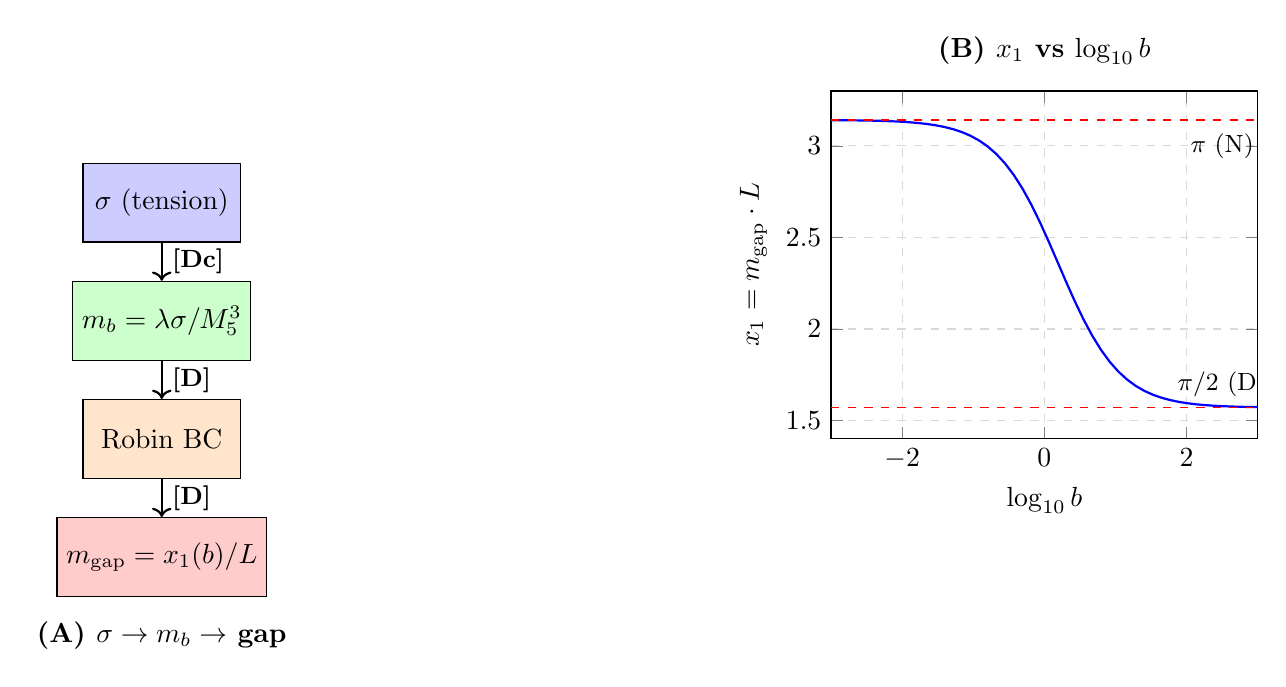
\begin{tikzpicture}
% Panel A: Schematic
\begin{scope}[xshift=0cm]
\node[draw, rectangle, minimum width=2cm, minimum height=1cm, fill=blue!20] (sigma) at (0,3) {$\sigma$ (tension)};
\node[draw, rectangle, minimum width=2cm, minimum height=1cm, fill=green!20] (mb) at (0,1.5) {$\mb = \lambda\sigma/\Mfive^3$};
\node[draw, rectangle, minimum width=2cm, minimum height=1cm, fill=orange!20] (robin) at (0,0) {Robin BC};
\node[draw, rectangle, minimum width=2cm, minimum height=1cm, fill=red!20] (gap) at (0,-1.5) {$\mgap = x_1(b)/L$};

\draw[->, thick] (sigma) -- (mb) node[midway, right] {\small \tagDc{}};
\draw[->, thick] (mb) -- (robin) node[midway, right] {\small \tagD{}};
\draw[->, thick] (robin) -- (gap) node[midway, right] {\small \tagD{}};

\node at (0, -2.5) {\textbf{(A) $\sigma \to \mb \to$ gap}};
\end{scope}

% Panel B: Graph
\begin{scope}[xshift=8.5cm]
\begin{axis}[
    width=7cm, height=6cm,
    title={\textbf{(B) $x_1$ vs $\log_{10} b$}},
    xlabel={$\log_{10} b$},
    ylabel={$x_1 = \mgap \cdot L$},
    xmin=-3, xmax=3,
    ymin=1.4, ymax=3.3,
    domain=-3:3,
    samples=50,
    grid=major,
    grid style={dashed, gray!30},
]
% Interpolating curve (approximate)
\addplot[blue, thick] {3.1416 * (1 + 10^x/3.1416)/(1 + 2*10^x/3.1416)};
% Asymptotes
\addplot[dashed, red] coordinates {(-3, 3.1416) (3, 3.1416)};
\addplot[dashed, red] coordinates {(-3, 1.5708) (3, 1.5708)};
% Labels
\node at (axis cs:2.5, 3.0) {\small $\pi$ (N)};
\node at (axis cs:2.5, 1.7) {\small $\pi/2$ (D)};
\end{axis}
\end{scope}
\end{tikzpicture}
\caption{(A) Schematic showing how brane tension $\sigma$ generates the mass gap through
$\mb = \lambda\sigma/\Mfive^3$ and Robin boundary conditions. Tags indicate derivation status.
(B) First eigenvalue $x_1$ as a function of $\log_{10} b$, transitioning from Neumann limit
($x_1 = \pi$) to Dirichlet limit ($x_1 = \pi/2$).}
\label{fig:sigma-to-gap}
\end{figure}

% ============================================================
% SECTION 9: COMPARISON WITH EW SCALE (COMPARISON ONLY)
% ============================================================
\section{Comparison with Electroweak Scale}
\label{sec:comparison}

\textbf{Note}: This section is \emph{comparison only}. The electroweak identification
is \tagI{}+\tagBL{}, not a derivation.

\subsection{Current Identification}

In the BLOCK-003 program, the gap is identified with $\MZ$:
\begin{equation}
\mgap = \MZ = 91.19\GeV \quad \tagI{}+\tagBL{}
\label{eq:gap-MZ}
\end{equation}

This implies:
\begin{equation}
L = \frac{\pi\hbar c}{\MZ} = 6.80 \times 10^{-18}\,\mathrm{m} \quad \tagI{}+\tagBL{}
\label{eq:L-from-MZ}
\end{equation}

\subsection{Implied $b$ Value}

Using this $L$ and the bridge relation:
\begin{equation}
\Mfive = \left(\frac{\Mpl^2}{L}\right)^{1/3} = 5.56 \times 10^{12}\GeV
\label{eq:M5-numerical}
\end{equation}

The brane mass is:
\begin{equation}
\mb = \frac{x_1}{L} - \frac{\pi}{L} \cdot (\text{correction from Robin})
\label{eq:mb-numerical}
\end{equation}

If the gap equals exactly $\pi/L$ (Neumann), then $\mb = 0$.
If there is a Robin correction:
\begin{equation}
\mgap = \frac{x_1(b)}{L} < \frac{\pi}{L}
\label{eq:gap-robin}
\end{equation}

\subsection{Matching Condition}

For the gap to equal $\MZ$ with a Robin BC:
\begin{equation}
\frac{x_1(b)}{L} = \MZ
\label{eq:matching}
\end{equation}

This requires:
\begin{equation}
x_1(b) = \MZ \cdot L = \MZ \cdot \frac{\pi\hbar c}{\MZ'} = \pi \cdot \frac{\MZ}{\MZ'}
\label{eq:matching-2}
\end{equation}

If $\MZ' = \MZ$ (self-consistent identification), then $x_1 = \pi$ (Neumann).

For Robin with $b > 0$, we need $x_1 < \pi$, implying $\mgap < \pi/L$,
which would give a gap smaller than the Neumann value.

\textbf{Conclusion}: The pure Neumann case ($\mb = 0$) is compatible with
$\mgap = \MZ$ if $L = \pi\hbar c/\MZ$. Robin corrections would modify this.

% ============================================================
% SECTION 10: EPISTEMIC LEDGER
% ============================================================
\section{Epistemic Ledger}
\label{sec:ledger}

\subsection{What Is Fixed}

\begin{table}[htbp]
\centering
\caption{Fixed quantities in the $\mb$-$\sigma$ relation.}
\label{tab:fixed}
\begin{tabular}{@{}llll@{}}
\toprule
Quantity & Expression & Status & Tag \\
\midrule
Dimensional scaling & $\mb \propto \sigma/\Mfive^3$ & Derived & \tagD{} \\
Bridge relation & $\Mpl^2 = \Mfive^3 L$ & Derived & \tagD{} \\
Spectral equation & $\tan(x_n) = -b/x_n$ & Derived & \tagD{} \\
Gap bounds & $\pi/2L < \mgap < \pi/L$ & Derived & \tagD{} \\
$b = \mb L$ & $b = \lambda\sigma L^2/\Mpl^2$ & Derived with $\lambda$ & \tagDc{} \\
\bottomrule
\end{tabular}
\end{table}

\subsection{What Is Open}

\begin{table}[htbp]
\centering
\caption{Open quantities requiring further input.}
\label{tab:open}
\begin{tabular}{@{}llll@{}}
\toprule
Quantity & Current Status & Required Input & Tag \\
\midrule
$\lambda$ & Undetermined & Topological constraint? & \tagOPEN{} \\
$\sigma$ & External or EDC-derivable & EDC dynamics? & \tagBL{} or \tagDc{} \\
$L$ & Identified with $\pi\hbar c/\MZ$ & Internal derivation? & \tagI{}+\tagBL{} \\
$\mgap$ & Identified with $\MZ$ & Above closures needed & \tagI{}+\tagBL{} \\
\bottomrule
\end{tabular}
\end{table}

\subsection{Path to GDC-2 (Calibrated Derivability)}

To achieve \tagDc{} for the gap:
\begin{enumerate}
\item Fix $\lambda$ (e.g., $\lambda = \pi$ from topological argument) \tagP{}$\to$\tagD{}
\item Express $\sigma$ in terms of $\Mpl$ (if possible) \tagBL{}$\to$\tagDc{}
\item Express $L$ in terms of $\Mpl$ (currently NO-GO from v16)
\end{enumerate}

\subsection{Path to GDC-1 (Full Derivability)}

To achieve \tagD{} for the gap:
\begin{enumerate}
\item All of GDC-2 requirements
\item No external mass scale (even $\Mpl$) in the final expression
\end{enumerate}

This is extremely challenging and likely impossible within current EDC.

% ============================================================
% SECTION 11: CONCLUSIONS
% ============================================================
\section{Conclusions}
\label{sec:conclusions}

\subsection{Summary of Results}

\begin{enumerate}
\item \textbf{Dimensional relation established}:
\begin{equation}
\mb = \lambda \, \frac{\sigma}{\Mfive^3} \quad \tagDc{}
\label{eq:conc-mb}
\end{equation}

\item \textbf{Dimensionless control parameter}:
\begin{equation}
b = \mb L = \lambda \, \frac{\sigma L^2}{\Mpl^2} \quad \tagDc{}
\label{eq:conc-b}
\end{equation}

\item \textbf{Topological pinning candidate}: $\lambda = \pi n$ or $2\pi n$ \tagP{}

\item \textbf{Connection to v26 spectrum}: $\tan(x_n) = -b/x_n$ with
$b = \lambda\sigma L^2/\Mpl^2$

\item \textbf{Gap status}: Remains \tagI{}+\tagBL{} until $\lambda$ and $L$ are fixed
\end{enumerate}

\subsection{What This Note Achieves}

\begin{itemize}
\item Maps how $\mb$ arises from $\sigma$ (dimensional + action-level)
\item Identifies $\lambda$ as the key undetermined coefficient
\item Proposes topological quantization as a candidate mechanism
\item Shows where the gap ``closes'' in parameter space
\end{itemize}

\subsection{What This Note Does NOT Achieve}

\begin{itemize}
\item Does not determine $\lambda$
\item Does not derive $L$ from EDC-internal principles
\item Does not upgrade gap to \tagD{} or \tagDc{}
\end{itemize}

\subsection{Next Steps (for P36+)}

\begin{enumerate}
\item Investigate specific topological mechanisms that could fix $\lambda$
\item Explore whether $\sigma$ can be expressed in terms of $\alpha$ or other EDC-derivables
\item Consider warped geometry where $L$ and $k$ might be related
\end{enumerate}

% ============================================================
% APPENDICES
% ============================================================
\appendix

\section{Detailed Dimensional Analysis}
\label{app:dimensional}

\subsection{All Possible Combinations}

With available quantities $\sigma$, $\Mfive$, $L$, $\Mpl$, we list all combinations
giving dimension $[M^1]$:

\begin{align}
\frac{\sigma}{\Mfive^3} &: \quad M^4/M^3 = M \label{eq:app-1} \\
\sigma L^3 &: \quad M^4 \cdot M^{-3} = M \label{eq:app-2} \\
\frac{\Mpl^2}{L^2 \Mfive} &: \quad M^2 \cdot M^2 / M = M \label{eq:app-3} \\
\Mfive &: \quad M \label{eq:app-4} \\
\Mpl &: \quad M \label{eq:app-5} \\
\frac{1}{L} &: \quad M \label{eq:app-6}
\end{align}

\subsection{Using the Bridge Relation}

With $\Mpl^2 = \Mfive^3 L$, we can express $\Mfive$ and $L$ in terms of each other:
\begin{equation}
\Mfive = \left(\frac{\Mpl^2}{L}\right)^{1/3}
\label{eq:app-M5-from-L}
\end{equation}

\begin{equation}
L = \frac{\Mpl^2}{\Mfive^3}
\label{eq:app-L-from-M5}
\end{equation}

Substituting \cref{eq:app-L-from-M5} into $\sigma/\Mfive^3$:
\begin{equation}
\mb = \lambda \frac{\sigma}{\Mfive^3} = \lambda \frac{\sigma L}{\Mpl^2}
\label{eq:app-mb-alternate}
\end{equation}

\subsection{Alternative Representations of $b$}

The control parameter $b = \mb L$ can be written:
\begin{equation}
b = \lambda \frac{\sigma L^2}{\Mpl^2} = \lambda \frac{\sigma L}{\Mfive^3} = \lambda \frac{\sigma \Mpl^2}{\Mfive^6}
\label{eq:app-b-forms}
\end{equation}

Each form emphasizes different physical content:
\begin{align}
\frac{\sigma L^2}{\Mpl^2} &: \quad \text{brane tension relative to 4D gravity at scale } L \label{eq:app-b-interp1} \\
\frac{\sigma L}{\Mfive^3} &: \quad \text{brane-induced coupling in 5D gravity} \label{eq:app-b-interp2} \\
\frac{\sigma \Mpl^2}{\Mfive^6} &: \quad \text{hierarchy between 4D and 5D gravity} \label{eq:app-b-interp3}
\end{align}

The combination $\sigma/\Mfive^3$ is preferred because:
\begin{itemize}
\item It involves only brane ($\sigma$) and bulk ($\Mfive$) scales
\item It does not require knowing $L$ a priori
\item It arises naturally from the gravitational coupling
\end{itemize}

\section{Action Derivation Details}
\label{app:action}

\subsection{Brane-Bulk Coupling}

The coupling between bulk field $\Phi$ and brane tension can be modeled as:
\begin{equation}
S_{\mathrm{int}} = -\int d^4x \sqrt{-\gamma} \, \sigma(\Phi) \delta(\xi - L)
\label{eq:app-interaction}
\end{equation}

where $\sigma(\Phi) = \sigma_0 + \sigma_1 \Phi + \frac{1}{2}\sigma_2\Phi^2 + \ldots$

\subsection{Quadratic Coupling}

The quadratic term gives:
\begin{equation}
S_{\mathrm{quad}} = -\frac{1}{2}\int d^4x \sqrt{-\gamma} \, \sigma_2 \, \Phi^2\big|_{\xi=L}
\label{eq:app-quad}
\end{equation}

Identifying $\mb = \sigma_2$, we need $[\sigma_2] = M$.

If $\sigma_2 \propto \sigma/\Mfive^3$, we recover \cref{eq:mb-primary}.

\subsection{Junction Condition Derivation}

From the Israel junction conditions with $\Phi$-dependent tension:
\begin{equation}
[K] = -\kappa_5^2 \sigma(\Phi)
\label{eq:app-junction}
\end{equation}

Expanding:
\begin{equation}
[K] = -\kappa_5^2 \sigma_0 - \kappa_5^2 \frac{d\sigma}{d\Phi}\Phi - \frac{1}{2}\kappa_5^2 \frac{d^2\sigma}{d\Phi^2}\Phi^2 + \ldots
\label{eq:app-junction-expanded}
\end{equation}

The $\Phi^2$ term contributes to the effective brane mass.

\section{Numerical Implementation}
\label{app:numerical}

\subsection{Root-Finding Algorithm}

The transcendental equation $f(x) = \tan(x) + b/x = 0$ is solved using:
\begin{enumerate}
\item Bracket the first root in $(\pi/2, \pi)$
\item Apply Brent's method for robust convergence
\item Verify residual $|f(x_1)| < 10^{-12}$
\end{enumerate}

The function to solve:
\begin{equation}
f(x) = \tan(x) + \frac{b}{x} = 0
\label{eq:app-f-def}
\end{equation}

Its derivative for Newton refinement:
\begin{equation}
f'(x) = \sec^2(x) - \frac{b}{x^2}
\label{eq:app-f-deriv}
\end{equation}

\subsection{Asymptotic Approximations}

For small $b$, the perturbation expansion:
\begin{equation}
x_1 = \pi - \frac{b}{\pi} - \frac{b^2}{\pi^3} + O(b^3)
\label{eq:app-small-b}
\end{equation}

For large $b$, the asymptotic series:
\begin{equation}
x_1 = \frac{\pi}{2} + \frac{\pi}{2b} - \frac{\pi^3}{8b^3} + O(b^{-5})
\label{eq:app-large-b}
\end{equation}

\subsection{Error Bounds}

The residual after root-finding:
\begin{equation}
\epsilon = |f(x_1)| = \left|\tan(x_1) + \frac{b}{x_1}\right| < 10^{-12}
\label{eq:app-residual}
\end{equation}

\subsection{Python Code Reference}

See \texttt{recompute.py} for:
\begin{itemize}
\item \texttt{find\_root(b)}: Returns $x_1$ for given $b$
\item \texttt{scan\_b(b\_range)}: Scans $b$ and returns $(b, x_1)$ pairs
\item \texttt{discrete\_lambda(n\_range)}: Computes for $\lambda = \pi n$
\end{itemize}

% ============================================================
% END DOCUMENT
% ============================================================

\end{document}
